\chapter{Przegląd badań na temat niezbalansowanych i zmiennych strumieni danych}

\noindent W niniejszym rozdziale dokonano przeglądu badań oraz literatury na temat niezbalansowanych oraz zmiennych strumieni danych. Ponadto zostaną szczegółowo wytłumaczone pojęcia podstawowe konieczne do zrozumienia dalszej części pracy. Temat eksploracji strumieni danych rozwinął się znacząco w ostatnich latach. Na rynku jest widocznych coraz więcej nowych narzędzi skupiających się na przetwarzaniu strumieni danych. Do najbardziej znanych i popularnych możemy zaliczyć:

\begin{itemize}
    \item \textit{Massive Online Analysis (MOA)} - środowisko do implementowania oraz testowania algorytmów eksploracji strumieni danych, zawiera sporo algorytmów strumieniowych oraz pozwala na łatwe implementowanie nowych \cite{Article:MOA}
    \item \textit{River} - biblioteka służąca do przetwarzania strumieni danych w języku Python \cite{Article:River}
    \item \textit{SAMOA} - jest to rozproszona wersja środowiska MOA, zawiera nie tylko algorytmy, ale również łatwe API i narzędzia do testowania i porównywania algorytmów \cite{Article:Samoa}
    \item \textit{Apache Flink} - narzędzie umożliwiające eksplorację strumieni danych w wersji rozproszonej, określany jako ,,następca'' Sparka, posiada moduły do integracji np. z Kafką, Flume czy Twitterem \cite{Article:Flink}
\end{itemize}

\noindent Każde z zaprezentowane narzędzi posiada oddaną, swoją rzeszę użytkowników, którzy poprzez swój wkład wpływają na rozwój narzędzi do przetwarzania strumieni danych. Wraz z rozwojem narzędzi nie mogło także zabraknąć rozwoju pod kątem coraz to bardziej zaawansowanych implementacji algorytmów działających w środowisku strumieniowym. Stosując coraz to nowsze podejścia użytkownicy starają się o ciągłą poprawę swoich wyników klasyfikacji oraz o zniwelowanie wartości czynników, które negatywnie wpływały na wartość końcową klasyfikacji. 

Przegląd prac naukowych dotyczących klasyfikacji niezbalansowanych i zmiennych strumieni danych posłużył do wstępnej selekcji algorytmów przetwarzania strumieniowego, które można by było rozszerzyć w taki sposób, aby radziły sobie z dodatkowymi trudnościami opisanymi w pracy \cite{Article:TypyPrzykladow}.

Najczęściej przejawiającym się algorytmem w analizowanych artykułach naukowych był \textit{Online Bagging} oraz wszelkie jego odmiany i rozszerzenia \cite{Article:TypyPrzykladow}\cite{Article:ManyAlgorithms}\cite{Article:OBFirst}\cite{Article:OBSecond}, co ukierunkowało naturalny wybór przetestowania i próby rozszerzenia tego algorytmu w opisywanej pracy. Warto także wspomnieć, że modyfikacje tego algorytmu charakteryzowały się wysokimi wynikami predykcji w stosunku do innych algorytmów opisywanych w innych publikacjach. Wybrane algorytmy przetwarzania strumieniowego zostały szczegółowo opisane w sekcji \ref{Teoria:Algorytmy}.

W ramach poniższej analizy oraz w celu zdefiniowania poniższych pojęć założono, że strumień danych może zostać zdefiniowany jako sekwencja elementów $S = \{x_t, y_t\}^{T}_{t=1}$, gdzie $x_t \in X$, $y_t \in Y$, $X$ w tym przypadku oznacza przestrzeń wielowymiarową o liczbie wymiarów równej liczbie atrybutów opisującej dany przykład (\english{input space}). W analizie będziemy skupiać się głównie na klasyfikacji binarnej, z tego względu $Y$ możemy zdefiniować jako zbiór $\{0,1\}$ (\english{output space}). Każdy z przykładów $(x_t, y_t)$ ma także przypisaną wartość z łącznego rozkładu prawdopodobieństwa strumienia opisaną jako $p_t(x,y)$ w chwili $t$ \cite{Article:TypyPrzykladow}. Założono także, że etykieta danego przykładu jest dostępna w momencie pojawienia się danego elementu w strumieniu.

\section{Dane niezbalansowane}

\noindent Dobór odpowiedniego algorytmu uczenia maszynowego może być nie tylko podyktowany jego wykorzystaniem we wszelakich, wcześniej omawianych pracach naukowych, ale także posiadanymi danymi i ich strukturą. W tematyce uczenia maszynowego wyszczególniamy dwa rodzaje danych: dane zbalansowane oraz dane niezbalansowane \cite{Article:Inz}.

Dane zbalansowane w tematyce eksploracji strumieni danych charakteryzują się tym, że przez cały okres napływania przykładów liczność elementów dla każdej z klas jest podobna - można powiedzieć, że każda z klas w dowolnym momencie działania algorytmu jest równoliczna.

Z kolei dane niezbalansowane w tematyce eksploracji strumieni danych są natomiast przeciwieństwem pojęcia danych zbalansowanych. Oznacza to, że gdy w analizowanym problemie klasyfikacji występują różne częstości pojawiania się obiektów należących do różnych klas, to problem taki należy traktować jako problem niezbalansowany - liczności klas w takim przypadku nie są równoliczne \cite{Article:Inz}.

Istotą problemu powyższego niezbalansowania jest przesłanka, że zastosowanie klasycznych mechanizmów uczenia na niezrównoważonym zbiorze danych może prowadzić do faworyzowania przez wyuczony klasyfikator klasy dominującej kosztem klasy zdominowanej. Innymi słowy, typowe podejście może skutkować skonstruowaniem modelu równoważnemu klasyfikatorowi, który przydziela wszystkim obiektom klasę dominującą, niezależnie od wartości wektora cech. Ze względu na zdecydowanie wyższą częstość pojawiania się obiektów z klasy dominującej w stosunku do klasy zdominowanej metoda charakteryzująca się niskim błędem klasyfikacji może charakteryzować się niskim (bądź zerowym) stopniem wykrywalności obserwacji z klasy zdominowanej \cite{MZieba}.

\label{Label:ImbalanceData}
W analizowanych przykładach strumień danych będzie oznaczony jako niezbalansowany w sytuacji, gdy w dowolnym momencie czasu $t$ zachodzi warunek $p_t(0) \ll p_t(1)$ lub $p_t(1) \ll p_t(0)$, gdzie $p_t(x)$ oznacza prawdopodobieństwo wystąpienia danego przykładu z klasy $x$ w chwili $t$. Klasa, która zawiera mniej przykładów jest nazywana klasą mniejszościową, natomiast z drugiej strony klasa zawierająca więcej przykładów nazywana jest klasą większościową. Aby określić globalny współczynnik niezbalansowania w strumieniu danych zdecydowano się na wykorzystanie wzoru $|S_{min}|/|S| * 100\%$, gdzie $|S_{min}|$ oznacza zaobserwowaną liczbę przykładów z klasy mniejszościowej, a $|S|$ oznacza zaobserwowaną ogólnę liczbę przykładów z wszystkich klas.

W niniejszej rozprawie problem niezbalansowania danych także występuje, przez co istnieje konieczność rozważenia jak sobie z nim poradzić. W celu uzyskania pełniejszego obrazu, bardziej szczegółowe wyjaśnienie dotyczące tego, jak algorytmy przetwarzania strumieni danych radzą sobie z problemem niezbalansowania danych, zostanie zaprezentowane w sekcji \ref{Teoria:Algorytmy}.


\section{Dryf pojęć}

\noindent Poza danymi niezbalansowanymi drugą składową tematu pracy są tzw. zmienne strumienie danych. Jak wcześniej wspomniano, za zmiany w strumieniu danych odpowiedzialne jest zjawisko nazywane dryfem pojęć (\english{concept drift}), które możemy zdefiniować jako zmiany definicji klas przewidywanych przez model w czasie.

Formalnie możemy opisać, że zjawisko dryfu pojęć wystąpiło w analizowanym strumieniu danych, jeśli dla dwóch różnych punktów w czasie $t$ i $t + \triangle$ warunek $\exists x : p_t(x, y) \ne p_{t + \triangle}(x, y)$ jest spełniony \cite{Article:DriftGama}\cite{Article:DriftGama2}.

Aby lepiej przedstawić to zjawisko posłużono się poniższą ilustracją:

\begin{figure}[h] 
    \centering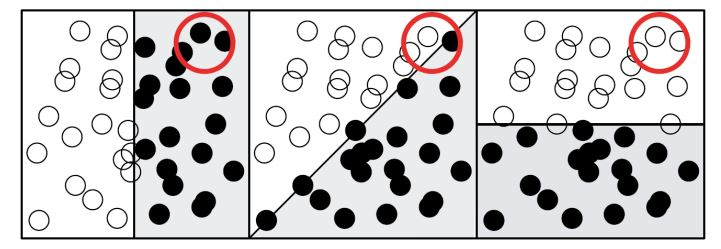
\includegraphics[width=14cm]{figures/concept_drift_example.JPG}
    \caption{Przykładowe zjawisko dryfu pojęć na przykładzie klasyfikacji binarnej \cite{DBrzezinski:Prezentacja}}
\end{figure}

\noindent Powyższy rysunek rozważa problem klasyfikacji binarnej. Na samym początku analizy strumienia można wyznaczyć granicę decyzyjną między klasami, która modelowana jest przez pionową linię przechodzącą przez środek. Wraz z upływem czasu można zauważyć jak wcześniej zamodelowana granica decyzyjna zmienia się. W środkowej części ilustracji można zauważyć, że nie jest to już pionowa linia, a linia która skierowana jest po ukosie. Na końcu analizy strumienia granica decyzyjna jeszcze uległa zmianie i zamodelowana została jako linia pozioma przechodząca przez środek. Przez zaprezentowanie tego przykładu można dostrzec jak zmieniały się definicje klas przewidywanych przez model w czasie.

\subsection{Rodzaje dryfu ze względu na zmianę prawdopodobieństwa}

\noindent Na podstawie informacji zawartych w poprzedniej sekcji wiadomo, że dryf pojęć odnosi się do zmian w prawdopodobieństwie predykcji danej klasy w dwóch różnych momentach w czasie. W pracy \cite{Article:Kelly} zaprezentowano podejścia według których zjawisko dryfu pojęć może zajść w analizowanym strumieniu. Podejścia te odnoszą się do:

\begin{itemize}
    \item Zmian w prawdopodobieństwach wystąpień klas (prawdopodobieństwo a priori) - $p(y)$
    \item Zmian w prawdopodobieństwach wystąpień danego przykładu - $p(x)$
    \item Zmian w rozkładzie przykładów - $p(x|y)$
    \item Zmian w prawdopodobieństwach warunkowych klas (prawdopodobieństwo a posteriori) - $p(y|x)$
\end{itemize}

\noindent Ze względu na przyczynę i skutek opisanych zmian wyróżnia się dwa rodzaje dryfu \cite{Article:DriftGama2}:

\begin{itemize}
    \item Dryf rzeczywisty (\english{real drift})
    \item Dryf wirtualny (\english{virtual drift})
\end{itemize}

\noindent Dryf rzeczywisty (\english{real drift}) można zdefiniować jako dryf odnoszący się do zmian w prawdopodobieństwach warunkowych klas $p(y|x)$. Co warte zaznaczenia, taka zmiana może wystąpić bez ingerencji w prawdopodobieństwa wystąpień klas $p(y)$ oraz w prawdopodobieństwa wystąpień danego przykładu $p(x)$. Takie rozróżnienie jest niezwykle istotne, ponieważ niektóre metody eksploracji strumieni danych próbują wykrywać zjawisko dryfu pojęć wykorzystując wyłącznie wartości atrybutów \cite{Article:RealDrift}. Obecność dryfu rzeczywistego w strumieniu danych wpływa na przesuwanie się granic decyzyjnych pomiędzy klasami w miarę upływu czasu związanego z analizą.

Dryf wirtualny (\english{virtual drift}) należy zdefiniować jako dryf odnoszący się do zmian w prawdopodobieństwach wystąpień klas $p(y)$ lub w prawdopodobieństwach wystąpień danego przykładu $p(x)$. Warty wyszczególnienia jest fakt, że ten rodzaj dryfu nie wpływa na prawdopodobieństwa warunkowe klas $p(y|x)$, które pozostają niezmienne przez cały okres klasyfikacji danych ze strumienia \cite{Article:VirtualDrift}. Obecność dryfu wirtualnego w strumieniu nie powoduje zjawiska przesuwania się granic decyzyjnych pomiędzy klasami w miarę upływu czasu.

\newpage

Aby lepiej przedstawić i zrozumieć różnicę między tymi dwoma rodzajami posłużono się poniższą ilustracją:

\begin{figure}[h] 
    \centering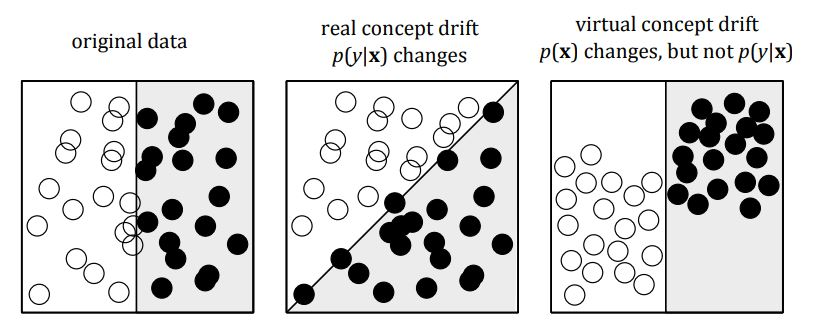
\includegraphics[width=14cm]{figures/types_of_drift.JPG}
    \caption{Rodzaje dryfu pojęć na przykładzie klasyfikacji binarnej \cite{Article:DriftGama2}}
\end{figure}

\noindent Powyższy rysunek rozważa problem klasyfikacji binarnej. Na samym początku analizy można wyznaczyć granicę decyzyjną między klasami, która modelowana jest przez pionową linię przechodzącą przez środek. Kolejne dwie ilustracje (środkowa i po prawej) modelują rozkład danych w sytuacji, gdy wystąpił odpowiednio dryf rzeczywisty oraz dryf wirtualny. W przypadku dryfu rzeczywistego należy zauważyć jak zmiana w prawdopodobieństwach warunkowych klas $p(y|x)$ wpływa na zmianę granicy decyzyjnej pomiędzy klasami. Końcowo granica decyzyjna zostaje zamodelowana nie przez pionową linię przechodzącą przez środek, ale przez linię skierowaną na ukos. W przypadku dryfu wirtualnego należy zwrócić uwagę przede wszystkim na fakt, że zmiana w prawdopodobieństwach wystąpień danego przykładu $p(x)$ nie wpływa na zmianę granicy decyzyjnej pomiędzy klasami. Granica została zamodelowana w identyczny sposób jak dla danych z początku analizy strumienia.

\subsection{Rodzaje dryfu ze względu na sposób zmiany}

\noindent Kolejnym niemniej ważnym aspektem opisującym dryf pojęć jest sposób zmiany. Zjawisko dryfu pojęć można scharakteryzować ze względu na np. trwałość, dotkliwość, przewidywalność czy częstotliwość zmian \cite{Article:DriftType}\cite{Article:DriftType2}. Jednak najbardziej analizowanym aspektem dryfów jest sposób, w jaki przejawiają się one w czasie \cite{Article:DriftGama}\cite{Article:DriftType3}.

\newpage

\begin{figure}[h] 
    \centering
    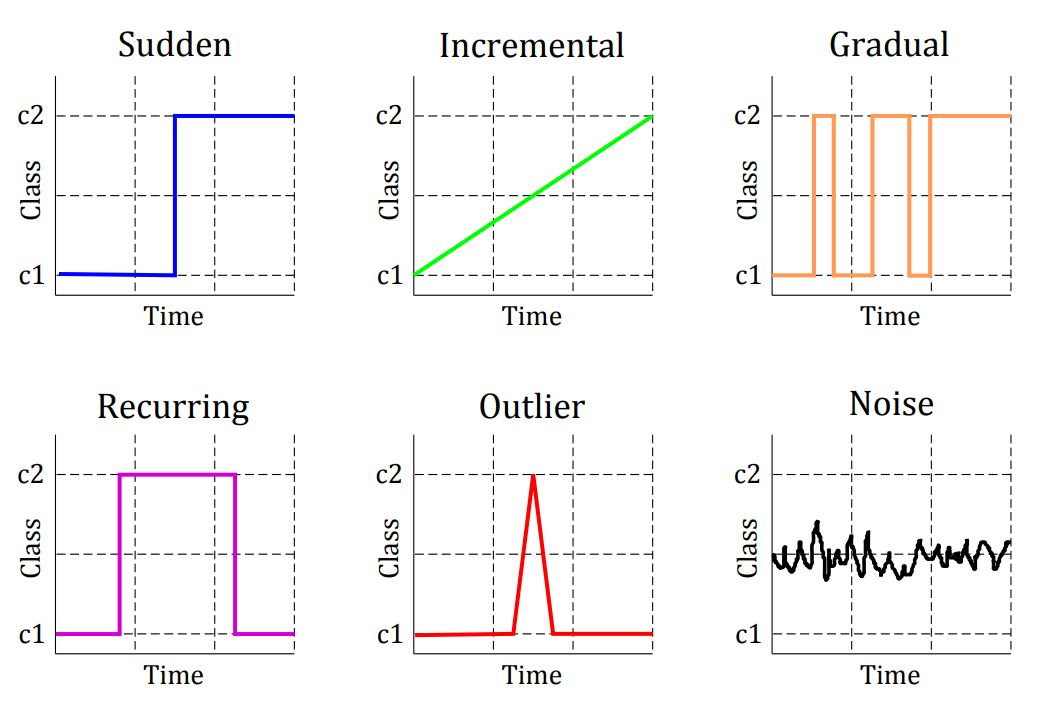
\includegraphics[width=14cm]{figures/types_of_drift2.JPG}
    \caption{Rodzaje typów zmian zachodzących w analizie strumieni danych \cite{Article:DriftType4}}\label{Figure:DriftTypes}
\end{figure}

\noindent Na rysunku \ref{Figure:DriftTypes} przedstawiono sześć podstawowych typów zmian, które mogą wystąpić w analizie poszczególnego strumienia danych w miarę upływu czasu. Pierwszy z wykresów (\textit{Sudden}) jest odwzorowaniem nagłej i nieodwracalnej zmiany, która wpływa na natychmiastową zmianę przypisania elementów do klas. Kolejne dwa wykresy (\textit{Incremental} oraz \textit{Gradual}) są przykładem zmiany, która zachodzi w wolniejszym tempie, aniżeli to było dla przypadku wykresu \textit{Sudden}. Dla zmiany \textit{Incremental} można zaobserwować stałe, wolne tempo zmiany, które też można określić jako ciąg drobnych zmian. Typ \textit{Gradual} natomiast odnosi się w tym przypadku do zmiany w rozkładzie prawdopodobieństw pojawiania się kolejnych przykładów. Kolejny typ oznaczony jako \textit{Recurring} odnosi się do tymczasowej, krótkotrwałej i nagłej zmiany. W miarę upływu czasu sytuacja wraca do stanu początkowego. Warta podkreślenia jest kwestia, że ten typ zmiany nie jest określony jako cykliczny i dla badacza nie jest to potwierdzone, kiedy taka zmiana nastąpi ponownie. Fakt ten stanowi główną różnicę w porównaniu do zjawiska sezonowości wykorzystywanej w statystyce \cite{PHD:Zliobaite}. Typ oznaczony jako \textit{Outlier} reprezentuje pojedynczy, rzadki przypadek zmiany w danych generowane przez źródło. Ostatni z typów oznaczony jako \textit{Noise} reprezentuje losowe, niewielkie zmiany, które tak naprawdę nie są związane ze żadną zmianą w danych generowane przez źródło. Warto zwrócić uwagę na kwestię, że w przetwarzaniu strumieniowym nie powinno reagować się na typy oznaczone jako \textit{Outlier} oraz \textit{Noise} z tego względu, że reprezentują losowe, nie wnoszące pozytywnego aspektu do analizy zmiany. Wspomniane typy przy analizie strumieni danych powinny zostać zignorowane \cite{DBrzezinski}\cite{Prezentacja:Strumienie}.

\subsection{Rodzaje dryfu ze względu na rozkład danych}
\label{Section:DriftDataDistribution}

\noindent Ostatnim aspektem, na który warto zwrócić uwagę przy przedstawianiu zjawiska dryfu pojęć, są zmiany szczególnie związane z rozkładem danych. Ostatnio dokonane badania naukowe zidentyfikowały kluczowe własności danych, które utrudniają proces uczenia się z danych niezbalansowanych.

Jedną z takich własności jest globalny współczynnik niezbalansowania (\english{global imbalance ratio}), zdefiniowany jako procent liczby przykładów należących do klasy mniejszościowej w stosunku do liczby wszystkich przykładów (sekcja \ref{Label:ImbalanceData}). Jednym z wniosków wyciągniętych na podstawie badań był fakt, że wysoka miara współczynnika niezbalansowania nie zawsze pogarszała wyniki klasyfikacji. Wniosek ten doprowadził badaczy do wyłonienia innych, kluczowych własności danych, nazywanych także \textit{czynnikami trudności danych} (\english{data difficulty factors}), które zostały zaklasyfikowane jako źródła pogorszenia trafności klasyfikatorów.

Skupiając się na literaturze skoncentrowanej na uczeniu z statycznych, niezbalansowanych danych, można wyszczególnić następujące czynniki trudności \cite{Book:DataDistribution}\cite{Article:DataDistribution}:

\begin{itemize}
    \item Dekompozycja klasy mniejszościowej na kilka mniejszych grup (\english{the decomposition of the minority class concept into several sub-concepts})
    \item Obecność małych, odizolowanych grup przykładów z klasy mniejszościowej zlokalizowanych w głębi grupy elementów klasy większościowej (\english{the presence of small, isolated groups of minority examples located deep inside the majority class region})
    \item Efekt silnego nakładania się przykładów z różnych klas (\english{the effect of strong overlapping between the classes})
\end{itemize}

\noindent Każdy z wymienionych czynników odgrywa swoją rolę także w przetwarzaniu strumieniowym. Warto także zwrócić uwagę na fakt, że wystąpienie kilku różnych czynników w strumieniu danych znacząco wpływa na trafność klasyfikacji, stąd istnieje konieczność opracowania algorytmów, które radziłyby sobie z wymienionymi trudnościami. Poza wspomnianymi czynnikami należy także skupić się na innych czynnikach, które nie są obecne w procesie uczenia z danych statycznych, a występują w procesie uczenia na strumieniu danych. Przykładem takich czynników występujących w przetwarzaniu strumieniowym są operacje związane ze zmianami położenia grup przykładów w przestrzeni atrybutów.\\\\
\textbf{Dekompozycja klasy mniejszościowej na kilka mniejszych grup}\\

\noindent Badania eksperymentalne z wykorzystaniem różnych, rzeczywistych zbiorów danych wykazały, że klasa mniejszościowa zwykle nie tworzy jednego, spójnego regionu w przestrzeni atrybutów, ale często jest rozproszona w mniejszych grupach rozsianych po całej przestrzeni \cite{Book:DataDistribution}\cite{Article:DataDistribution2}\cite{Inbook:DataDistribution}. Naukowcy rozpoczęli badania nad wpływem dekompozycji klas na wydajność popularnych klasyfikatorów na kilku syntetycznych zbiorach danych \cite{Article:DataDistribution}. W ich eksperymentach skupisko stworzone z elementów klasy mniejszościowej, początkowo otoczony przykładami klasy większościowej, było sukcesywnie dzielone na kilka mniejszych grup, które były oddzielone przez regiony klasy większościowej. Wyniki pokazały, że zwiększenie podziału klasy mniejszościowej miało większy wpływ na trafność klasyfikacji aniżeli zmiana globalnego współczynnika niezbalansowania, zwłaszcza w przypadku mniejszej liczby przykładów \cite{Article:TypyPrzykladow}.\\\\
\textbf{Obecność małych, odizolowanych grup przykładów z klasy mniejszościowej zlokalizowanych w głębi grupy elementów klasy większościowej}\\

\noindent Zwykle są to grupy par, trójek przykładów z klasy mniejszościowej zlokalizowane dość daleko od granic decyzyjnych swojej klasy. Przyjmując koncepcję opisaną w \cite{Article:DataDistribution3} grupy takie nazywa się rzadkimi przypadkami (\english{rare cases}) i ze względu na ich rzadkość różnią się one od większych skupisk opisanych w sekcji dotyczącej dekompozycji. Z racji faktu, że klasa mniejszościowa jest niedoreprezentowana, nie można tych elementów traktować jako szumu. Na co warto zwrócić uwagę to fakt, że badania \cite{Article:DataDistribution2} dowiodły, że rzadkie przykłady, jeśli zostaną odpowiednio potraktowane, np. poprzez przetwarzanie wstępne (\english{pre-processing}), mogą być wykorzystane do poprawy predykcji klasy mniejszościowej. Należy pamiętać, że również pojedyncze przykłady mniejszościowe mogą znajdować się wewnątrz klasy większościowej lub w regionie pustej przestrzeni odgrywając rolę wartości odstających (\english{outlier}). Poprawne rozpoznanie takich przypadków jest niezwykle trudne, a większość metod specjalistycznych traktuje takie wartości odstające jako szum, dlatego w dalszych eksperymentach nacisk zostanie położony na poprawne rozpoznawanie rzadkich przypadków \cite{Article:TypyPrzykladow}.\\\\
\textbf{Efekt silnego nakładania się przykładów z różnych klas}\\

\noindent Efekt silnego nakładania się przypadków związany jest z nakładaniem się regionów przykładów z klasy mniejszościowej i większościowej w przestrzeni atrybutów. Czynnik ten jest obecny w wielu rzeczywistych zbiorach danych, a szczegółowe badania eksperymentalne wykazały, że jego rola jest jeszcze bardziej znacząca w przypadku danych niezbalansowanych, a w szczególności w przypadku klasy mniejszościowej. Autorzy pracy \cite{Article:DataDistribution4} wykazali, że zwiększenie liczby nakładających się obszarów pogorszyło wydajność sześciu popularnych klasyfikatorów w znacznie większym stopniu niż zmiana współczynnika niezbalansowania. Ponadto zaobserwowali oni także większy wypływ lokalnego współczynnika niezbalansowania w regionie nakładania się przykładów z różnych klas \cite{Article:TypyPrzykladow}.

\begin{figure}[h] 
    \centering
    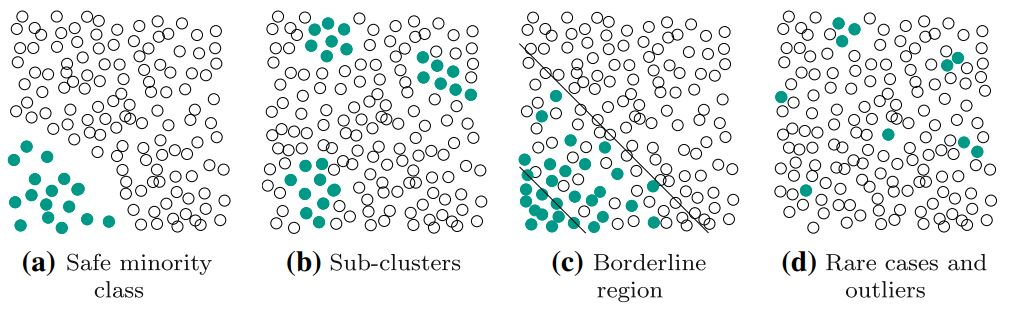
\includegraphics[width=15cm]{figures/data_examples.JPG}
    \caption{Prezentacja rozkładów danych klasy mniejszościowej z określonymi czynnikami trudności \cite{Article:TypyPrzykladow}}\label{Figure:TypesExample}
\end{figure}

\noindent Na rysunku \ref{Figure:TypesExample} można zaobserwować graficzne odwzorowanie wszystkich wymienionych czynników. Klasa mniejszościowa na rysunku oznaczona jest kolorem zielonym. Na ilustracji \textbf{(a)} nie mamy do czynienia z czynnikami trudności, klasa mniejszościowa jest logicznie odseparowana od klasy większościowej. Przypadek \textbf{(b)} ilustruje sytuację dekompozycji klas mniejszościowej na kilka mniejszych skupisk, rozmieszczonych w kilku miejscach w przestrzeni atrybutów. Przypadek \textbf{(c)} pokazuje sytuację efektu silnego nakładania się przykładów z różnych klas. W celu ułatwienia interpretacji region nakładania się został wyszczególniony poprzez zaznaczenie jego granic dwoma linia. Ostatni z rysunków \textbf{(d)} przedstawia sytuację istnienia rzadkich oraz odstających przypadków z klasy mniejszościowej zlokalizowanych w głębi grupy elementów klasy większościowej. Jak można zauważyć grupy te są zdecydowanie mniejsze aniżeli te oznaczone na ilustracji \textbf{(b)} i najczęściej liczą dwa, trzy elementy (przypadki rzadkie) lub pojedyncze elementy (przypadki odstające).\\\\
\textbf{Rodzaje przykładów z klasy mniejszościowej ze względu na ich lokalne sąsiedztwo}\\

\noindent Analiza wspomnianych czynników trudności danych prowadzi do wyróżnienia różnych typów przykładów klasy mniejszościowej na podstawie liczby znajdujących się w ich pobliżu przykładów klasy mniejszościowej oraz większościowej \cite{Article:DataDistribution3}. Jedno z podejść do rozróżniania typów przykładów z klasy mniejszościowej \cite{Article:DataDistribution3}\cite{Article:DataDistribution2} analizuje etykiety klas przykładów w ich lokalnym sąsiedztwie zdefiniowanym przez k-najbliższych sąsiadów. W tym podejściu przykład z danej klasy oznaczany jest jako:

\begin{itemize}
    \item Bezpieczny (\english{safe}) - jeśli większość jego sąsiadów należy do tej samej klasy
    \item Brzegowy (\english{borderline}) - jeśli liczba etykiet sąsiadów z obu klas jest podobna
    \item Odstający (\english{outlier}) - jeśli wszyscy jego sąsiedzi należą do przeciwnej klasy
    \item Rzadki (\english{rare}) - jeśli liczba jego sąsiadów znajduje się pomiędzy granicami poziomu przypadku odstającego i brzegowego
\end{itemize}

\noindent Zaletą przyjęcia takiej konwencji przykładów bezpiecznych, brzegowych, odstających i rzadkich jest kwestia, że w ten sposób możliwe jest określenie udziału każdego typu przykładów z klasy mniejszościowej w procesie klasyfikacji na rzeczywistych zbiorach danych \cite{Article:TypyPrzykladow}\cite{Article:DataDistribution3}\cite{Article:DataDistribution2}.\\\\
\textbf{Zmiana pozycji grup obiektów}\\

\noindent Ostatnim z czynników trudności, który zostanie zaprezentowany, jest czynnik związany ze zmianą pozycji grup przykładów w przestrzeni atrybutów w miarę upływu czasu. Warta podkreślenia jest kwestia, że czynnik ten nie ma prawa wystąpić w analizie statycznych zbiorów danych ze względu na ich stałą, niezmienną strukturę. W przypadku strumieni danych rozważa się środowisko dynamiczne, w którym może dochodzić do zmian definicji klas przewidywanych przez model w czasie. W dotychczasowych pracach związanych nad analizą skupień w strumieniach danych próbowano modelować i monitorować ewolucję (przejścia) skupisk w czasie \cite{Article:ClusterTransition}. Przejścia te możemy podzielić na zewnętrzne i wewnętrzne.

\begin{itemize}
    \item Przejścia zewnętrzne - mogą być skategoryzowane jako podział skupiska na wiele mniejszych skupisk, zniknięcie skupiska, pojawienie się lub wchłonięcie przez inny skupisko
    \item Przejścia wewnętrzne - dotyczą jednego określonego skupiska, który może się rozszerzyć lub skurczyć w miarę upływu czasu, zmiana może także dotyczyć przesunięcia się środka skupiska lub całkowitej zmiany jego rozmieszczenia w przestrzeni atrybutów
\end{itemize}

\noindent Poprawne zamodelowanie oraz śledzenie zmian skupisk w analizie strumieni danych wpływa pozytywnie na ogólną trafność klasyfikacji, dlatego ważnym elementem w procesie projektowania algorytmu jest skupienie się na opisanym czynniku.

\section{Sposoby przetwarzania strumieni danych}

\noindent W dzisiejszym ujęciu analizy strumieni danych wyszczególniamy dwa podejścia przetwarzania strumieni danych. Pierwsze podejście skupia się na pojedynczym przetwarzaniu przykład po przykładzie w określonych momentach w czasie i jest określane przetwarzaniem przyrostowym (\english{online processing}). Celem drugiego podejścia jest przetwarzanie elementów strumienia w partiach, blokach o równym rozmiarze. Podejście takie jest określane przetwarzaniem blokowym (\english{block processing}).

\subsection{Przetwarzanie przyrostowe}

\begin{figure}[h] 
    \centering
    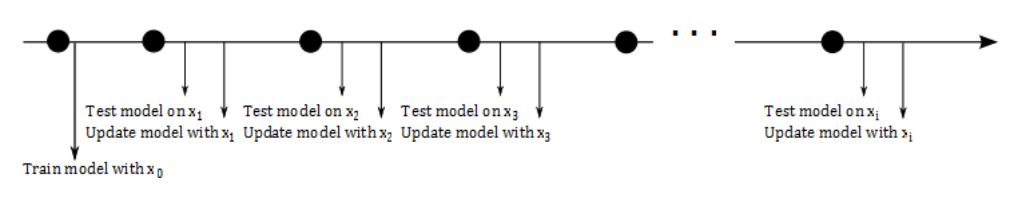
\includegraphics[width=15cm]{figures/online_processing.JPG}
    \caption{Proces uczenia ze strumienia danych w przetwarzaniu przyrostowym \cite{BrzezPhd2015}}\label{Figure:OnlineProcessing}
\end{figure}

\noindent Na rysunku \ref{Figure:OnlineProcessing} przedstawiono proces uczenia ze strumienia danych w przetwarzaniu przyrostowym. Tak jak wspomniano wcześniej, w tym podejściu każdy pojedynczy przykład zostaje przetworzony przez algorytm w momencie pojawienia się w strumieniu. Podejście to skupia się na przetwarzaniu przykład po przykładzie. Warto także zwrócić uwagę na okoliczność, że w momencie pojawienia się przykładu, najpierw wykonywana jest faza testowania modelu, a dopiero później model zostaje uaktualniony o wiedzę o tym przykładzie (faza uczenia). Taka ewaluacja nazywana jest oceną \textit{Test-then-train} i zostanie szczegółowo przedstawiona w sekcji \ref{Secton:TestThenTrain}.

\newpage

\subsection{Przetwarzanie blokowe}

\begin{figure}[h] 
    \centering
    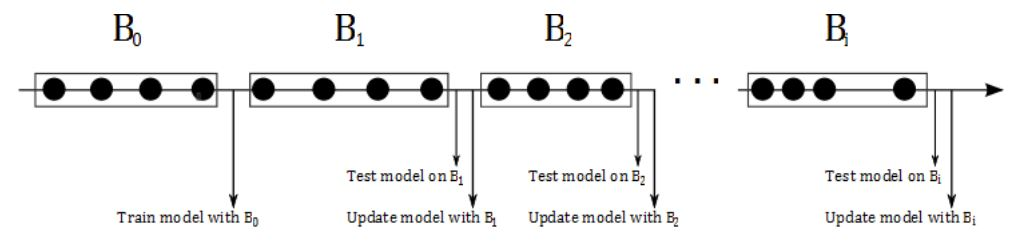
\includegraphics[width=15cm]{figures/block_processing.JPG}
    \caption{Proces uczenia ze strumienia danych w przetwarzaniu blokowym \cite{BrzezPhd2015}}\label{Figure:BlockProcessing}
\end{figure}

\noindent Na rysunku \ref{Figure:BlockProcessing} przedstawiono proces uczenia ze strumienia danych w przetwarzaniu blokowym. Tak jak wspomniano wcześniej, celem tego podejścia jest przetwarzanie elementów strumienia w partiach, blokach o równym rozmiarze. Po zgromadzeniu odpowiedniej liczby przykładów w bloku danych, partia taka, podobnie jak to było we wcześniejszym podejściu, poddana zostaje najpierw fazie testowania na aktualnym modelu, a dopiero później następuje faza uczenia, gdzie model zostaje rozszerzony o dodatkową wiedzę pochodzącą z aktualnie przetworzonego bloku danych.

\noindent Warto także zwrócić uwagę na okoliczność, że przetwarzanie przyrostowe może zostać potraktowane jako szczególny przypadek przetwarzania blokowego, w którym wielkość każdego bloku $|B_j| = 1$

\section{Sposoby oceny algorytmów strumieniowych}

\noindent Eksploracja strumieni danych wymaga zdefiniowania własnych, oddzielnych sposóbów oceny algorytmów aniżeli te, które są znane z uczenia tradycyjnego. W uczeniu statycznym głównym podejściem, które jest najczęściej stosowane to podział zbioru danych na zbiór treningowy, testowy oraz walidacyjny. Dodatkowym czynnikiem, który często jest wykorzystywany przy ocenie algorytmów w środowisku statycznym jest wykonanie oceny krzyżowej (\english{cross-validation}). W środowisku dynamicznym nie jest możliwy fizyczny podział zbioru danych na zbiór treningowy, testowy oraz walidacyjny ze względu na nieograniczoność przypadków, które mogą pojawić się w takim strumieniu. Ponadto, tak jak to zostało wcześniej przedstawione, nie możliwe jest przechowywanie wszystkich przypadków, które pojawiły się w strumieniu, przez cały okres działania algorytmu, ze względu na ograniczoną pamięć. Dodatkowo w środowisku strumieniowym nie jest możliwe odtworzenie operacji oceny krzyżowej, z tego względu, że operacja taka jest zbyt kosztowna obliczeniowo - ograniczenie dotyczące czasu przetwarzania. Ze względu na restrykcje, które nakłada środowisko strumieniowe, powstało wiele specjalizowanych sposobów oceny algorytmów strumieniowych, które mają za zadanie ułatwić sprawdzenie trafności klasyfikacji dokonywanej na elementach strumienia.

\newpage

\subsection{Holdout}

\begin{figure}[h] 
    \centering
    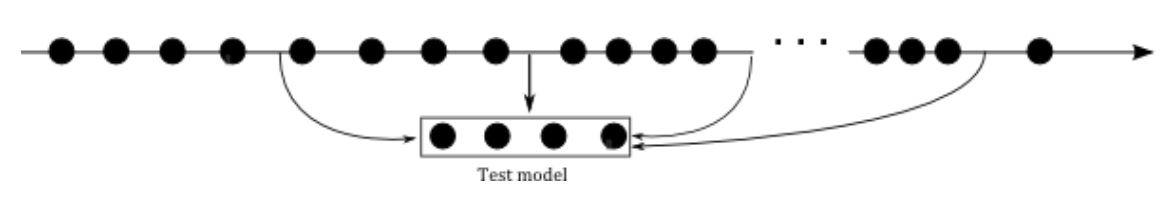
\includegraphics[width=15cm]{figures/holdout.JPG}
    \caption{Sposób oceny algorytmów strumieniowych - \textbf{Holdout} \cite{Prezentacja:Strumienie}}\label{Figure:Holdout}
\end{figure}

\noindent Pierwszym z zaprezentowanych sposobów oceny algorytmów strumieniowych jest podejście \textit{Holdout}, zaprezentowane na rysunku \ref{Figure:Holdout}. Podejście to stara się być odwzorowaniem podziału na zbiór treningowy i testowy, znanego z uczenia statycznego. W tym sposobie tworzony jest niezależny zbiór testowy, do którego trafiają wybrane przykłady ze strumienia danych. Na podstawie tak stworzonego zbioru testowego dokonywana jest ocena procesu klasyfikacji na badanym strumieniu danych. Proces ten jest cykliczny, kolejne sprawdzenia dokonywane są na tym samym zbiorze testowym co określoną liczbę przykładów, które pojawią się w strumieniu (np. co milion przykładów) \cite{PHD:Kirkby}. Ze względu na stałą reprezentację zbioru testowego, metoda ta nie powinna być wykorzystywana do oceny strumieni danych, gdzie występuje dryf pojęć. Możliwość zmian w strumieniu powoduje, że przykłady znajdujące się w zbiorze testowym mogą być przestarzałe i nie powinny być wykorzystywane do oceny klasyfikatora.

\subsection{Test-Then-Train}
\label{Secton:TestThenTrain}

\begin{figure}[h] 
    \centering
    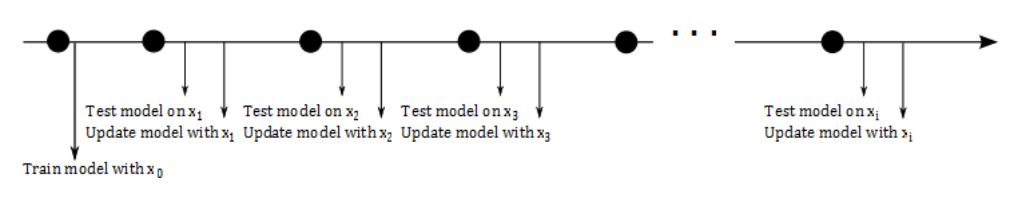
\includegraphics[width=15cm]{figures/online_processing.JPG}
    \caption{Sposób oceny algorytmów strumieniowych - \textbf{Test-Then-Train} \cite{Prezentacja:Strumienie}}\label{Figure:TestThenTrain}
\end{figure}

\noindent Drugim z zaprezentowanych sposobów oceny algorytmów strumieniowych jest podejście \textit{Test-Then-Train}, zaprezentowane na rysunku \ref{Figure:TestThenTrain}. Tak jak opisywano wcześniej, przy szczegółowym przedstawieniu sposobu przetwarzania przyrostowego, podejście to charakteryzuje się wykonaniem procesu testowania modelu na nowym przykładzie i następnie późniejszą fazą uczenia modelu na podstawie danych z nowego przykładu. Warto podkreślić fakt, że technika ta nie wymaga dodatkowej pamięci koniecznej na przechowywanie przykładów zbioru testowego. Metoda ta może być w pełni wykorzystywana do każdego rodzaju strumieni danych \cite{PHD:Kirkby}.

\subsection{Block-Based Evaluation}

\begin{figure}[h] 
    \centering
    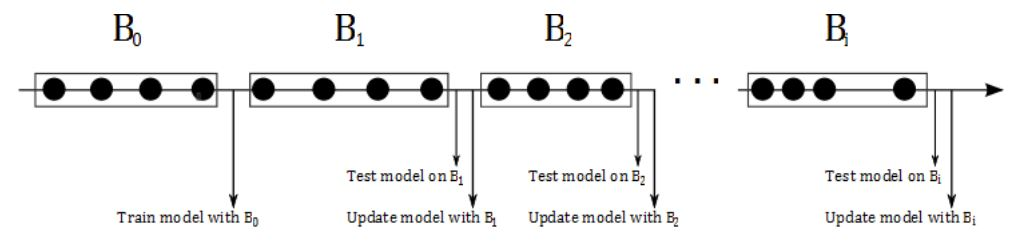
\includegraphics[width=15cm]{figures/block_processing.JPG}
    \caption{Sposób oceny algorytmów strumieniowych - \textbf{Block-Based Evaluation} \cite{Prezentacja:Strumienie}}\label{Figure:BlockBasedEvaluation}
\end{figure}

\noindent Trzecim z zaprezentowanych sposobów oceny algorytmów strumieniowych jest podejście \textit{Block-Based Evaluation}, zaprezentowane na rysunku \ref{Figure:BlockBasedEvaluation}. Podejście to charakteryzuje się tym, że łączy cechy dwóch wcześniej opisanych sposobów. Trafność klasyfikacji oceniania jest nie na pojedynczych przykładach, tylko na blokach danych, a schemat działania jest ten sam, co w przypadku sposobu \textit{Test-Then-Train}. W pierwszej kolejności wykonywana jest faza testowania modelu na nowym bloku danych, po czym następuje faza uczenia modelu o nową wiedzę zawartą w przykładach w bloku. Metoda ta także może być w pełni wykorzystywana do każdego rodzaju strumieni danych \cite{DBrzezinski}.

\subsection{Prequential}

\begin{figure}[h] 
    \centering
    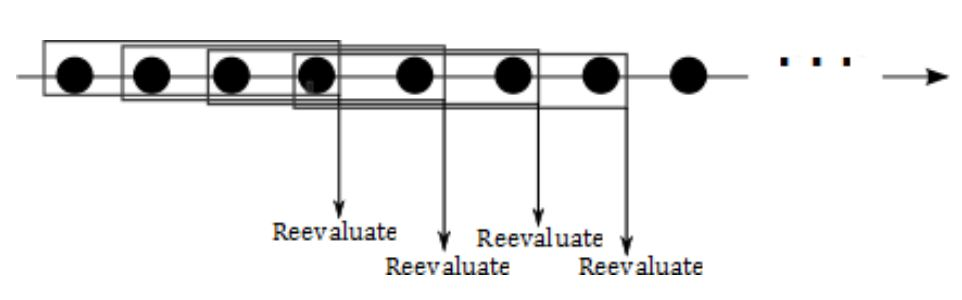
\includegraphics[width=15cm]{figures/prequential.JPG}
    \caption{Sposób oceny algorytmów strumieniowych - \textbf{Prequential} \cite{Prezentacja:Strumienie}}\label{Figure:Prequential}
\end{figure}

\noindent Ostatnim z zaprezentowanych sposobów oceny algorytmów strumieniowych jest podejście \textit{Prequential}, zaprezentowane na rysunku \ref{Figure:Prequential}. Podejście to także stara się wykorzystać cechy wcześniej opisanych sposobów oraz dodatkowo wprowadza swoje własne modyfikacje. Jedną z takich modyfikacji jest widoczna na rysunku metoda uczenia z wykorzystaniem okna przesuwnego (\english{sliding window}). Okno przesuwne w ocenie strumieni danych zawiera określoną liczbę najświeższych przykładów, które pojawiły się w strumieniu. Po pojawieniu się w strumieniu nowego przykładu, następuje usunięcie z okna przykładu najstarszego i ponowna ewaluacja trafności klasyfikacji. Kolejnym elementem, które wprowadza to podejście, jest współczynnik związany z zapominaniem najstarszych przykładów w oknie (\english{fading factor}). Współczynnik ten sprawia, że przykładom starszym, znajdującym się w oknie, zostaje przypisana niższa waga, aniżeli przykładom, które do tego okna niedawno trafiły. W ten sposób większy nacisk jest położony na naukę z najświeższych danych \cite{Article:Evaluation}.

\section{Miary oceny algorytmów strumieniowych}

\noindent W niniejszej sekcji przedstawione zostaną miary oceny, którymi możemy się posłużyć przy ocenie klasyfikatorów działających na strumieniach danych. W odróżnieniu od zaprezentowanych w poprzedniej sekcji sposobów oceny, tak w przypadku miar ocen algorytmów strumieniowych istnieje możliwość posłużenia się popularnymi miarami, które wykorzystuje się przy uczeniu z danych statycznych. Aby lepiej przedstawić najbardziej znane miary oceny zaprezentowana została poniższa macierz pomyłek dla problemu klasyfikacji binarnej:

\begin{center}
\begin{table}[h]
\renewcommand{\arraystretch}{1.5}
\label{tab:macierz}
\begin{center}
\begin{tabular}{|c|c|c|c|}
   \cline{3-4} 
   \multicolumn{1}{c}{} & & \multicolumn{2}{c|}{Predicted} \\ \cline{3-4}
   \multicolumn{1}{c}{} & & Positive & Negative \\ \hline
   
   {Observed}
   & Positive & TP & FN \\ \cline{2-4}
   & Negative & FP & TN  \\ \cline{2-4} \hline
\end{tabular}
\caption{Macierz pomyłek dla problemu klasyfikacji binarnej}
\end{center}
\end{table}
\end{center}

\noindent Założono, że klasa oznaczona jako \textit{Positive} oznacza klasę mniejszościową, podczas gdy klasa oznaczona jako \textit{Negative} oznacza klasę większościową. Wartości \textit{TP (True Positive)} oraz \textit{TN (True Negative)} oznaczają przypadki, w których klasyfikator dokonał poprawnej predykcji odpowiednio dla przykładu z klasy mniejszościowej i większościowej. Wartości \textit{FN (False Negative)} oraz \textit{FP (False Positive)} oznaczają przypadki, w których klasyfikator zaklasyfikował niepoprawnie odpowiednio przykład z klasy mniejszościowej i większościowej. Wykorzystując wprowadzone wartości wyszczególniono poszczególne miary ocen dla algorytmów klasyfikacji \cite{Inbook:Metrics}:

$$\textrm{Accuracy = }\frac{TP + TN}{TP + TN + FP + FN}$$
$$\textrm{Precision = }\frac{TP}{TP + FP}$$
$$\textrm{Sensitivity (Recall) = }\frac{TP}{TP + FN}$$
$$\textrm{Specificity = }\frac{TN}{TN + FP}$$
$$\textrm{G-mean = }\sqrt{\frac{TP}{TP + FN} \cdot \frac{TN}{TN + FP}}$$\\

\noindent Powyżej zostały zaprezentowane najbardziej popularne miary, wykorzystywane przy ocenie klasyfikatorów w uczeniu z danych statycznych. Wszystkie te miary mogłyby zostać z powodzeniem wykorzystane przy ocenie algorytmów bazujących na strumieniach danych. Należałoby jednak zwrócić uwagę na kwestię, że w pracy rozważany jest problem poprawy klasyfikacji niezbalansowanych i zmiennych strumieni, wobec czego nie wszystkie miary zostaną rozważone w dalszej części rozprawy. Jedną z takich miar jest miara trafności (\english{accuracy}), która dla algorytmów, predykujących zawsze klasę większościową, działających na strumieniach danych, gdzie 99\% przypadków stanowią elementy z klasy większościowej, osiągnąć może maksymalną wartość 99\%. Doszłoby w takim przypadku do faworyzowania przez wyuczony klasyfikator klasy dominującej kosztem klasy zdominowanej.

Należy szczególnie uważać na wspomniane zjawisko dominowania przez klasyfikator jednej klasy wobec drugiej, dlatego w niniejszej pracy zwracana jest szczególna uwaga na miary:

\begin{itemize}
    \item Czułości (\english{sensitivity}), która przekazuje informację, jaki procent przypadków z klasy mniejszościowej został sklasyfikowany pozytywnie
    \item Swoistości (\english{specificity}), która przekazuje informację, jaki procent przypadków z klasy większościowej został sklasyfikowany poprawnie
    \item G-mean, która jest pierwiastkiem z iloczynu miar czułości i swoistości, co oznacza, że kładzie nacisk na poprawną klasyfikację przypadków z obu klas, przy czym reaguje silniej na zjawisko faworyzowania aniżeli miara dokładności
\end{itemize}

Wymienione powyżej miary są bardzo często nieodłącznym elementem prac naukowych związanych z analizą niezbalansowanych i zmiennych strumieni danych \cite{Article:TypyPrzykladow}\cite{Inbook:Metrics}\cite{Article:OBFirst}\cite{Article:OBSecond}, wobec czego wybór tych właśnie miar do analizy w niniejszej rozprawie był naturalny.

\section{Algorytmy przetwarzania strumieni danych}
\label{Teoria:Algorytmy}

\noindent Tematyka związana z eksploracją strumieni danych była i jest poruszana w wielu pracach naukowych. Wraz z upływem lat w środowisku osób zajmujących się strumieniami danych możemy zauważyć powstawanie coraz to innych, rozbudowanych podejść do projektowania algorytmów przetwarzania. Wprowadzone algorytmy i specjalne podejścia można podzielić na cztery główne kategorie:

\begin{itemize}
    \item Pojedyncze klasyfikatory (\english{single classifiers})
    \item Techniki bazujące na wykorzystaniu okna (\english{windowing techniques})
    \item Detektory dryfu (\english{drift detectors})
    \item Klasyfikatory złożone (\english{ensemble approaches})
\end{itemize}

\subsection{Pojedyncze klasyfikatory}

\noindent Pojedyncze klasyfikatory są szczególnie znane z eksploracji danych w środowiskach statycznych. Co warte podkreślenia klasyfikatory te mogą zostać dostosowane w taki sposób, aby radziły sobie ze zmieniającymi się strumieniami danych. Klasyfikatorom działającym na danych statycznych, mimo możliwości przetwarzania sekwencyjnego danych, brakuje mechanizmu adaptacyjnego w stosunku do eksploracji strumieni danych. Na szczęście klasyfikatory takie można zmodyfikować w łatwy sposób zmodyfikować, aby reagowały na zmiany w strumieniach \cite{BrzezPhd2015}. 

W ramach tej grupy możemy wyszczególnić pięć rodzajów algorytmów:

\begin{itemize}
    \item Sieci neuronowe (\english{Neural networks}) \cite{Article:NeuralNetworks}
    \item Naiwny klasyfikator Bayesa (\english{Naive Bayes}) \cite{Article:NaiveBayes}
    \item Klasyfikatory oparte na najbliższym sąsiedztwie (\english{Nearest neighbour classifiers}) \cite{Article:Neighbours}
    \item Klasyfikatory wykorzystujące reguły decyzyjne (\english{Rule learners}) \cite{Article:DecisionRules}
    \item Drzewa decyzyjne (\english{Decision trees})
\end{itemize}

\noindent W zakresie niniejszej rozprawy szczegółowo zostanie wyjaśniony algorytm drzewa Hoeffding'a (\english{Hoeffding tree}), który należy do ostatniej grupy algorytmów - drzew decyzyjnych.\\\\
\textbf{Drzewo Hoeffding'a}\\

\noindent Drzewo Hoeffding'a można zdefiniować jako algorytm drzewa decyzyjnego służący do klasyfikacji danych strumieniowych. W klasycznym algorytmie drzewa decyzyjnego nie ma problemu z określeniem najlepszego atrybutu podziału. W przetwarzaniu strumieniowym nie jest możliwe określenie najlepszego atrybutu podziału, ze względu na brak wszystkich danych i nieograniczone pojawianie się kolejnych przykładów. Główną ideą tego algorytmu jest hipoteza, że często mała próbka danych może wystarczyć do określenia najlepszego atrybutu podziału drzewa decyzyjnego. Drzewo Hoeffding'a zostało dostosowane do nauki na danych strumieniowych poprzez wprowadzenie granicy Hoeffding'a, którą możemy zdefiniować w następujący sposób \cite{BrzezPhd2015}:

\begin{equation}
    \epsilon = \sqrt{\frac{R^2ln(1/\delta)}{2n}}
\end{equation}

\noindent gdzie:

\begin{itemize}
    \item $R$ - zakres wartości estymowanej funkcji
    \item $\delta$ - dopuszczalny błąd estymacji
    \item $n$ - rozmiar próbki
\end{itemize}

\noindent Drzewo Hoeffding'a działa w następujących etapach: 

\begin{enumerate}
    \item Zebranie odpowiednich statystyk z próbki strumienia
    \item Estymacja wartości funkcji oceny podziału dla każdego atrybutu
    \item Wykorzystanie granicy Hoeffding'a do zagwarantowania wyboru atrybutu podziału
\end{enumerate}

\newpage

\begin{figure}[h] 
    \centering
    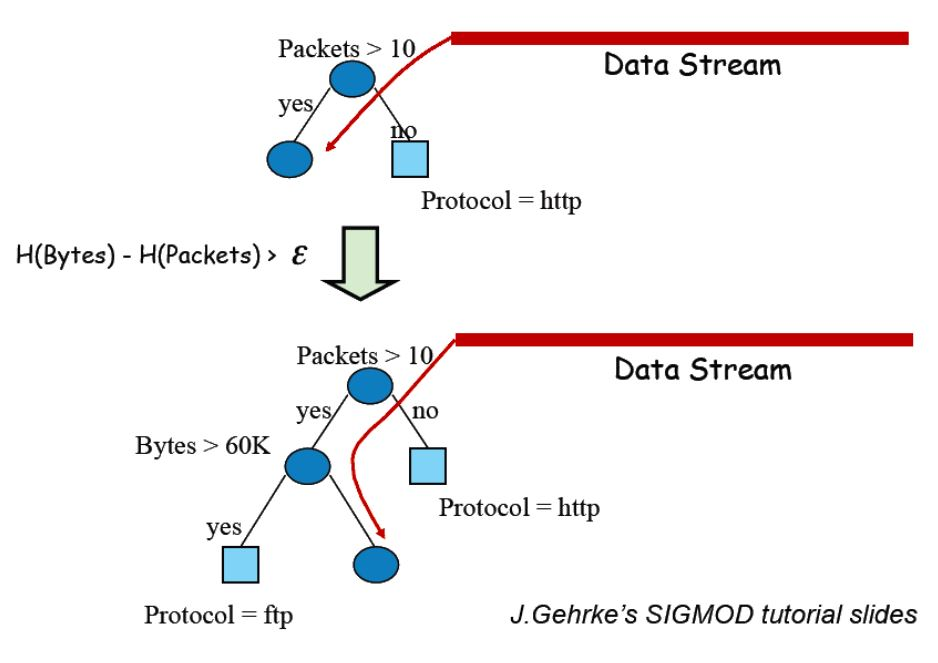
\includegraphics[width=15cm]{figures/hoeffding_tree.JPG}
    \caption{Przykład budowy drzewa Hoeffding'a \cite{Prezentacja:Strumienie}}\label{Figure:HoeffdingTree}
\end{figure}

\noindent Na podstawie rysunku \ref{Figure:HoeffdingTree} można zaobserwować przykładowy proces wyboru atrybutu podziału w drzewie Hoeffding'a. Po wykonaniu drugiego etapu (estymacji wartości funkcji oceny dla każdego atrybutu) algorytm jest w stanie wybrać dwie największe wartości funkcji oceny i sprawdzić czy różnica między nimi jest większa niż oszacowana wartość granicy Hoeffding'a. Jeśli różnica ta jest większa to tworzony jest w drzewie nowy warunek podziału, w przeciwnym razie drzewo pozostaje w niezmienionej formie. Warto też zwrócić uwagę na fakt, że granica Hoeffding'a jest prawdziwa dla dowolnego rozkładu danych, co oznacza, że badacz podczas eksploracji nie musi martwić się o to, żeby jego dane pochodziły np. z rozkładu normalnego czy dwumianowego.

Pojęcie granicy Hoeffding'a było ważnym aspektem w kontekście analizy strumieni danych i przyczyniło się do powstania jednego z bardzo znanych algorytmów w analizie strumieni danych - Very Fast Decision Tree (VFDT) \cite{Article:VFDT}. Analizując ten algorytm warto także zwrócić uwagę na pracę \cite{Article:Rutkowski}, która wykazała, że w pierwotnej propozycji algorytmu źle zastosowano zastosowano granicę Hoeffding'a. W tej samej pracy autorzy pokazali także, że ograniczenie Hoeffding'a może zostać zastąpione innymi rozwiązaniami pochodzącymi z probabilistyki, np. nierównością McDiarmida (\english{McDiarmid's inequality}) \cite{Article:Rutkowski}.

\subsection{Techniki bazujące na wykorzystaniu okna}

\noindent Wiele algorytmów do analizy strumieni danych wykorzystuje techniki opierające się na użyciu okna. Najczęściej pojawiającą się formą okna w literaturze są okna przesuwne (\english{sliding windows}). Zadaniem okna przesuwnego jest ograniczenie liczby przykładów, które biorą udział w procesie uczenia. Ponadto okno przesuwne dba o to, żeby były to zawsze najświeższe przykłady. Najstarsze przykłady są usuwane z okna po pojawieniu się nowych przykładów. Ważną własnością okien przesuwnych jest fakt, że za ich pomocą istnieje możliwość przetransformowania algorytmu ze środowiska statycznego do środowiska działającego na strumieniach danych.

\begin{algorithm}
    \caption{Basic windowing algorithm \cite{BrzezPhd2015}}\label{Algorithm:Window}
    \textbf{Input}: $S$: data stream of examples \\
    \hspace*{12mm} $W$: window of examples \\
    \textbf{Output}: $C$: a classifier built on examples in window $W$ \\
    \begin{algorithmic}[1]
    \State initialize window $W$
    \ForAll{examples $x^t \in S$ \do} 
    \State $W \gets W \cup \{x^t\}$
    \State if necessary remove outdated examples from $W$
    \State rebuild/update $C$ using $W$
    \EndFor
    \end{algorithmic}
\end{algorithm}

\noindent Podstawowa technika bazująca na wykorzystaniu okna przesuwnego została zaprezentowany w sekcji algorytmu \ref{Algorithm:Window}. Na podstawie pseudokodu można zauważyć, że okno przesuwne jest uzupełniane do momentu pełnego zapełnienia. W sytuacji, gdy okno przesuwne jest w pełni zapełnione, a w strumieniu pojawi się nowy przykład, to najstarszy przykład z okna zostaje usunięty, a jego miejsce zajmuje najświeższy przykład. Warto także zwrócić uwagę na kwestię, że klasyfikator jest odpowiednio przebudowywany po pojawieniu się nowego przykładu w strumieniu. Uaktualnienie modelu klasyfikatora odbywa się na podstawie danych z okna przesuwnego. Jednym z podstawowych problemów w tej technice jest dobranie odpowiedniego rozmiaru okna, zbyt mały rozmiar okna sprawi, że klasyfikator będzie reagował szybko na zmiany, ale może to spowodować spadek jego stabilności. Zbyt duży rozmiar okna z kolei może sprawić, że klasyfikator nie będzie w stanie odpowiednio reagować i przystosowywać się do zmian w strumieniu. Z tego też powodu technika ta jest rozszerzana o dodatkowe elementy jak np. manipulacja wielkości okna podczas działania algorytmu lub wprowadzenie współczynnika zapominania najstarszych przykładów w oknie - przypisanie im mniejszej wagi niż nowszym przykładom \cite{BrzezPhd2015}.

\subsection{Detektory dryfu}

\noindent Kolejnym z podejść stosowanym w analizie strumieni danych jest zastosowanie detektorów dryfu pojęć. Detektory dryfu, podobnie jak techniki bazujące na wykorzystaniu okna, także pozwalają na przetransformowanie dowolnego algorytmu ze środowiska statycznego do środowiska działającego na strumieniach danych \cite{Article:DriftGama2}. Główną ideą detektorów dryfu jest śledzenie błędu klasyfikatora i porównywanie tej wartości z wartością oczekiwaną odchylenia standardowego. Zwykle fakt ten sprawdza się poprzez skorzystanie z testów statystycznych, które sprawdzają czy aktualny błąd klasyfikatora lub rozkłady klas pozostają niezmienne w czasie.

\newpage

\begin{figure}[h] 
    \centering
    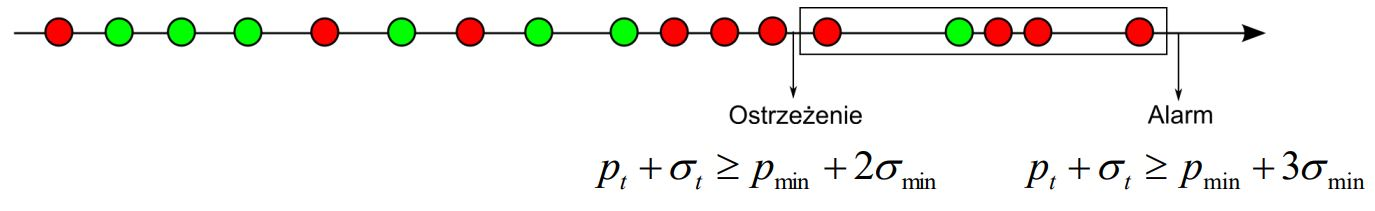
\includegraphics[width=15cm]{figures/drift_detection.JPG}
    \caption{Przykład zastosowania detektora dryfu (\textit{Drift Detection Method (DDM)}) w analizie strumienia danych \cite{Prezentacja:Strumienie}}\label{Figure:DriftDetection}
\end{figure}

\noindent Na rysunku \ref{Figure:DriftDetection} można zaobserwować przykładowe działanie detektora dryfu. Detektor ten posiada zdefiniowane dwa warunki, które oznaczają kolejno poziom ostrzeżenia oraz alarmu. W sytuacji, gdy warunek zdefiniowany jako poziom ostrzeżenia zostanie spełniony to algorytm zaczyna od tego momentu zbieranie nowych przykładów i przechowywanie ich w pamięci. Jeśli warunek zdefiniowany jako alarm zostanie spełniony to w tym momencie skonstruowany algorytm odrzuca dotychczasowy klasyfikator, na którym dokonywana była ocena danych ze strumienia i buduje nowy klasyfikator na przykładach zbieranych od momentu osiągnięcia stanu alarmowego (ostrzeżenia).

Do najbardziej popularnych algorytmów wykorzystujących detektor dryfu należą: \textit{Drift Detection Method (DDM)} \cite{Article:DriftDetection}, \textit{Early Drift Detection Method (EDDM)} \cite{Article:DriftDetection2}, \textit{Page-Hinkley Test} \cite{Article:PageHinkley}, \textit{ADWIN} \cite{Article:ADWIN}.

\subsection{Klasyfikatory złożone}

\noindent Ostatnie z zaprezentowanych podejść dotyczy klasyfikatorów złożonych (\english{ensemble classifiers}). Podejście to jest także wykorzystywane przy nauce ze statycznych zbiorów danych i jest powszechnym sposobem wykorzystywanym w celu polepszenia trafności klasyfikacji. Klasyfikatory złożone tak naprawdę stanowią zbiór pojedynczych klasyfikatorów, gdzie każdy pojedynczy klasyfikator nauczony zostaje z wykorzystaniem różnej próbki danych pobranej ze zbioru danych. Ostateczna decyzja, o tym jaka klasa zostanie przypisana nowemu przykładowi, zostaje podjęta często przy wykorzystaniu mechanizmu głosowania większościowego. Decyzja dokonana na podstawie zbioru klasyfikatorów jest często bardziej dokładna aniżeli decyzja dokonana na podstawie pojedynczego klasyfikatora. Ogólny schemat zastosowania klasyfikatora złożonego w procesie uczenia został przedstawiony w algorytmie \ref{Algorithm:Ensemlbe}.

\begin{algorithm}
    \caption{Generic ensemble training algorithm \cite{PHD:Kirkby}}\label{Algorithm:Ensemlbe}
    \textbf{Input}: $S$: set of examples \\
    \hspace*{12mm} $n$: number of classifiers in ensemble \\
    \textbf{Output}: $\mathcal{E}$: an ensemble of classifiers \\
    \begin{algorithmic}[1]
    \State $\mathcal{E} \gets n$ classifiers
    \ForAll{classifiers $C_i$ in ensemble $\mathcal{E}$ \do} 
    \State select a subset of examples $D_i$ from $S$
    \State build $C_i$ using $D_i$
    \EndFor
    \end{algorithmic}
\end{algorithm}

\noindent W przypadku analizy strumieni danych nie jest możliwe skorzystanie z całego zbioru danych ze względu na jego nieograniczoność, dlatego zaprezentowany schemat uczenia musi zostać odpowiednio dostosowany do działania w środowisku dynamicznym. Dodatkowym aspektem, na który należałoby zwrócić uwagę, jest zjawisko dryfu pojęć. Aby poradzić sobie odpowiednio ze zmianami w strumieniu można by było wprowadzić mechanizm zapominania przy projektowaniu algorytmu \cite{BrzezPhd2015}.

W zakresie grupy klasyfikatorów złożonych można wyszczególnić dwa podejścia:

\begin{itemize}
    \item \textit{Klasyfikatory przyrostowe} - uczą się na bieżąco przykład po przykładzie
    \item \textit{Klasyfikatory blokowe} - uczą się partiami na odpowiednio zebranych blokach danych
\end{itemize}

\noindent W ramach niniejszej rozprawy szczególną uwagę położono na  analizę i porównanie klasyfikatorów przyrostowych, które to klasyfikatory były podstawą do stworzenia nowych podejść starających się spełnić opisany cel rozprawy.\\\\
\textbf{Online Bagging}\\

\noindent Jednym z najbardziej znanych algorytmów należących do grupy klasyfikatorów złożonych, przyrostowych jest algorytm \textit{Online Bagging} zaprezentowany po raz pierwszy w pracy \cite{Article:OnlineBagging}. Algorytm ten jest modyfikacją oryginalnego algorytmu \textit{Bagging} zaproponowanego przez Breiman'a w 1996 roku. Pseudokod algorytmu \textit{Online Bagging} został przedstawiony w sekcji \ref{Algorithm:OnlineBagging}.

\begin{algorithm}
    \caption{Online Bagging \cite{Article:OnlineBagging}}\label{Algorithm:OnlineBagging}
    \textbf{Input}: $S$: stream of examples \\
    \hspace*{12mm} $n$: number of classifiers in ensemble \\
    \textbf{Output}: $\mathcal{E}$: an ensemble of classifiers \\
    \begin{algorithmic}[1]
    \State $\mathcal{E} \gets n$ incremental classifiers
    \ForAll{examples $x^t \in S$ \do}
    \ForAll{classifiers $C_i \in \mathcal{E}$ \do}
    \State set $l$ $\sim Poisson(1)$
    \For{1 to $l$ \do}
    \State update $C_i$ using $x^t$
    \EndFor
    \EndFor
    \EndFor
    \end{algorithmic}
\end{algorithm}

\noindent Na podstawie przedstawionego algorytmu \ref{Algorithm:OnlineBagging} można przeanalizować różnice między algorytmami działającymi w dwóch różnych środowiskach. Zasadniczą różnicą występującą w algorytmie \textit{Online Bagging} jest zmiana w podejściu do losowania przykładów, które mają zostać przekazane na wejście danemu klasyfikatorowi składowemu. W przypadku tradycyjnego algorytmu \textit{Bagging} możliwy jest do dyspozycji cały zbiór danych, na podstawie którego są tworzone próbki typu \textit{bootstrap} przekazywane na wejście danemu klasyfikatorowi składowemu. Próbki te tworzone są poprzez losowanie ze zwracaniem przykładów z oryginalnego zbioru danych. Takie podejście nie jest możliwe do zastosowania w wersji strumieniowej algorytmu ze względu na nieograniczoność przykładów. W zamian zdecydowano się skorzystać z rozkładu Poissona z parametrem rozkładu $\lambda$ = 1. 

W sytuacji, gdy w strumieniu pojawi się nowy przykład, następuje operacja aktualizacji klasyfikatorów składowych o dane zaprezentowane na nowym przykładzie. W tym momencie dla każdego z klasyfikatorów składowych losowana jest liczba z rozkładu Poissona, która, po wykonaniu operacji zaokrąglenia do liczby naturalnej, determinuje, ile razy dany przykład, który pojawił się w strumieniu ma zostać zaprezentowany danemu klasyfikatorowi składowemu. Losowanie z wykorzystaniem rozkładu Poissona stanowi odwzorowanie tradycyjnego losowania próbki \textit{bootstrap} z oryginalnego algorytmu \textit{Bagging}.

Warto zwrócić uwagę także na kwestię, że algorytm \textit{Online Bagging} nie zawiera takich mechanizmów jak np. mechanizm zapominania, wobec czego można wysunąć hipotezę, że algorytm ten nie będzie w stanie poradzić sobie z klasyfikacją niezbalansowanych i zmiennych strumieni danych. Hipoteza ta zostanie zweryfikowana na podstawie analizy wyników oceny eksperymentalnej zawartej w sekcji \ref{Section:Results}. Obserwacje te były także przyczyną do powstania rozszerzeń tego algorytmu, jak np. \textit{Undersampling Online Bagging (UOB)} oraz \textit{Oversampling Online Bagging (OOB)} \cite{Article:OBFirst}\cite{Article:OBSecond}.\\\\
\textbf{Undersampling Online Bagging i Oversampling Online Bagging}\\

\noindent Algorytmy \textit{Undersampling Online Bagging} oraz \textit{Oversampling Online Bagging} stanowią rozszerzenie wcześniej zaprezentowanego algorytmu \textit{Online Bagging}. Główną różnicą w tych podejściach jest zastosowanie techniki modyfikacji dostępnego zbioru danych poprzez dolosowywanie lub usuwanie przykładów ze zbioru uczącego (\english{resampling}). Można wyróżnić dwie główne techniki modyfikacji zbioru danych:

\begin{itemize}
    \item Undersampling - usuwanie przykładów klasy większościowej ze zbioru uczącego
    \item Oversampling - dolosowywanie przykładów klasy mniejszościowej do zbioru uczącego
\end{itemize}

\noindent Obie te modyfikacje mają na celu zbalansowanie zbioru uczącego w celu uniknięcia zjawiska faworyzowania klasy większościowej przez dany klasyfikator. W przypadku uczenia ze statycznego zbioru nie ma żadnych problemów ze swobodnym usuwaniem i dolosowywaniem przykładów do zbioru. W przypadku uczenia ze strumieni danych operacje te obsłużono za pomocą modyfikacji parametru $\lambda$ rozkładu Poissona.

\begin{figure}[h] 
    \centering
    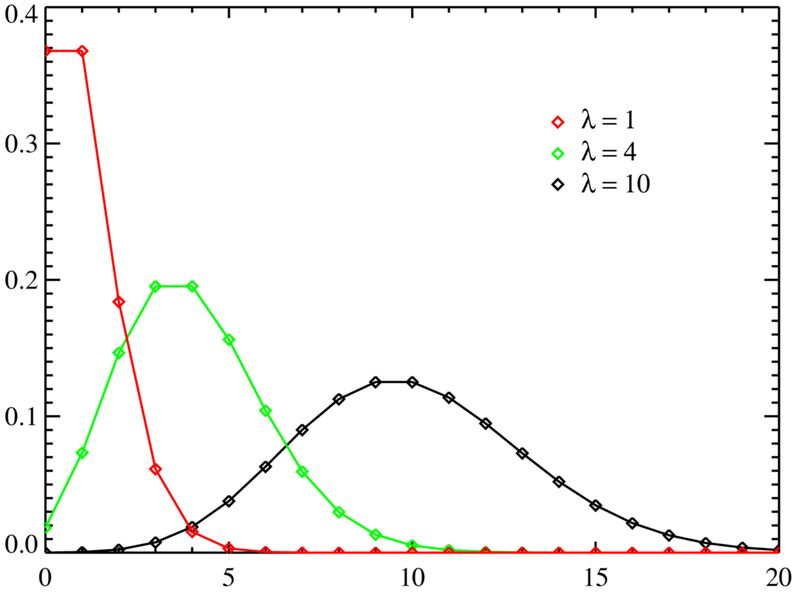
\includegraphics[width=7cm]{figures/poisson.JPG}
    \caption{Rozkład Poissona dla różnych wartości parametru $\lambda$}\label{Figure:Poisson}
\end{figure}

\noindent Jak można zauważyć na rysunku \ref{Figure:Poisson}, dla większych wartości parametru $\lambda$ rozkład Poissona generuje coraz to większe wartości i powoli zbiega do rozkładu normalnego. Dostrajając wartość $\lambda$ rozkładu Poissona użytkownik jest w stanie wymusić na algorytmie, aby dany element np. z klasy mniejszościowej był więcej razy pokazany danemu klasyfikatorowi aniżeli element z klasy większościowej. Obserwacja ta była przyczyną do powstania nowych odmian algorytmów bazujących właśnie na zjawisku \textit{resampling'u}.

\begin{algorithm}
    \caption{Undersampling and Oversampling Online Bagging \cite{Article:OBSecond}}\label{Algorithm:UOBOOB}
    \textbf{Input}: $S$: stream of examples \\
    \hspace*{12mm} $n$: number of classifiers in ensemble \\
    \textbf{Output}: $\mathcal{E}$: an ensemble of classifiers \\
    \begin{algorithmic}[1]
    \State $\mathcal{E} \gets n$ incremental classifiers
    \ForAll{examples $x^t \in S$ \do}
    \State update currenct class size $w^{(t)} = (w^{(t)}_{+}, w^{(t)}_{-})$
    \ForAll{classifiers $C_i \in \mathcal{E}$ \do}
    \vspace{0.4em}
    \If{$y_t$ = $+1$ and $
        \begin{cases}
            w^{(t)}_{+} < w^{(t)}_{-} \textrm{for OOB}\\
            w^{(t)}_{+} > w^{(t)}_{-} \textrm{for UOB}
        \end{cases}$}
    \vspace{0.5em}
    \State set $l$ $\sim Poisson(w^{(t)}_{-}/w^{(t)}_{+})$
    \vspace{0.5em}
    \ElsIf{$y_t$ = $-1$ and $
        \begin{cases}
            w^{(t)}_{-} < w^{(t)}_{+} \textrm{for OOB}\\
            w^{(t)}_{-} > w^{(t)}_{+} \textrm{for UOB}
        \end{cases}$}
        \vspace{0.5em}
    \State set $l$ $\sim Poisson(w^{(t)}_{+}/w^{(t)}_{-})$
    \Else
    \State set $l$ $\sim Poisson(1)$
    \EndIf
    \For{1 to $l$ \do}
    \State update $C_i$ using $x^t$
    \EndFor
    \EndFor
    \EndFor
    \end{algorithmic}
\end{algorithm}

\noindent W sekcji algorytmu \ref{Algorithm:UOBOOB} został zaprezentowany pseudokod pokazujący modyfikację parametru rozkładu $\lambda$ w zależności od działania w trybie \textit{undersampling'u} lub \textit{oversampling'u}. W pseudokodzie został poruszony problem klasyfikacji binarnej. Główną ideą obu rozszerzeń jest modyfikacja parametru $\lambda$ poprzez wykorzystanie wartości oznaczonych jako $w^{(t)}_{+}$ oraz $w^{(t)}_{-}$. Wartości te odpowiednio oznaczają procent przykładów, które należą do klasy oznaczonej jako $+$ w chwili $t$ oraz drugi procent przykładów, które należą do klasy oznaczonej jako $-$. Oznacza to, że oba rozszerzenia w ramach swojego działania śledzą zmieniające się liczności obu klas w czasie. Poniżej został zaprezentowany wzór, który jest odpowiedzialny za aktualizację liczności wszystkich klas po pojawieniu się nowego przykładu w strumieniu.

\begin{equation}
    w^{(t)}_k = \theta w^{(t-1)}_k + (1 - \theta)[(x_k, c_k)], (k = 1, ..., N)
\end{equation}

\noindent gdzie:

\begin{itemize}
    \item $[(x_k, c_k)] = 1$ jeżeli prawdziwą etykietą przykładu $x_t$ jest klasa $c_k$, w przeciwnym wypadku $[(x_k, c_k)] = 0$
    \item $\theta$ $(0 < \theta < 1)$ - predefiniowany współczynnik zapominania
\end{itemize}

\noindent Jak można zauważyć wspomniane rozszerzenia algorytmu \textit{Online Bagging} wprowadzają w swojej implementacji współczynnik zapominania oznaczony jako $\theta$. Współczynnik ten powoduje, że starsze dane mają mniejszy wpływ na obliczanie procentu przypadków danej klasy wraz z upływem czasu. Jest to zastosowanie pewnego rodzaju wygładzania wykładniczego \cite{Article:OBSecond}. Oba rozszerzenia poprzez śledzenie liczności przykładów danych klas odpowiednio manipulują wartością rozkładu $\lambda$, chcąc doprowadzić do poprawy klasyfikacji przykładów z klasy mniejszościowej.\\\\
\textbf{Weighted Ensemble of Undersampling Online Bagging and Oversampling Online Bagging}\\

\noindent Ostatnim z zaprezentowanych podejść dla klasyfikatorów złożonych jest podejście, które w swoim działaniu wykorzystuje dwa wcześniej wspomniane algorytmy \textit{UOB} oraz \textit{OOB}. W ramach ewaluacji na konkretnym strumieniu danych algorytm ten dokonuje procesu uczenia na obu algorytmach składowych, a końcowa ocena finalnej etykiety dla elementu, który pojawił się w strumieniu odbywa się na podstawie średniej ważonej miary \textit{G-mean}. W pracy \cite{Article:OBSecond} przedstawiono dwie różne strategie wykorzystania obu algorytmów składowych. Pierwsza strategia przypisuje odpowiednio obliczone wagi każdemu algorytmowi składowemu na podstawie aktualnej wartości miary \textit{G-mean}. Druga strategia polega na wykorzystaniu do procesu predykcji algorytmu, który w danym momencie w czasie posiada wyższą wartość miary \textit{G-mean}. Zakładając, że proces predykcji odbywa się na podstawie średniej ważonej obu algorytmów oraz, że parametry $\alpha_o$ oraz $\alpha_u$ oznaczają odpowiednio wagi algorytmów \textit{OOB} oraz \textit{UOB} można zdefiniować następujące własności:

\begin{itemize}
    \item Dla pierwszej strategii:
    \begin{equation}
        \alpha_o = \frac{g_o}{g_o + g_u}, \alpha_u = \frac{g_u}{g_o + g_u}
    \end{equation}
    \item Dla drugiej strategii:
    \begin{equation}
        \begin{cases}
        \alpha_o = 1, \alpha_u = 0 \hspace{4mm} \textrm{if} \hspace{2mm} g_o \geq g_u\\
        \alpha_o = 0, \alpha_u = 1 \hspace{4mm} \textrm{if} \hspace{2mm} g_o < g_u
        \end{cases}
    \end{equation}
\end{itemize}

\noindent gdzie:

\begin{itemize}
    \item $g_o$ - wartość miary \textit{G-mean} dla algorytmu \textit{OOB}
    \item $g_u$ - wartość miary \textit{G-mean} dla algorytmu \textit{UOB}
\end{itemize}

\noindent Ideą zastosowania takiego podejścia była kwestia dotycząca tego, że ze statystycznego punktu widzenia połączenie wyników kilku klasyfikatorów przez uśrednienie może zmniejszyć ryzyko wyboru klasyfikatora o słabych wynikach, a tym samym zapewnić zapewnić stabilne i dokładne wyniki. Zastosowane uśrednienie może, ale nie musi przewyższać wyników najlepszych klasyfikatorów składowych \cite{Article:Hybrid}\cite{Article:OBSecond}.